\chapter{Methodology}

\section{Review / Criticism}
\subsection{XText Grammar}
The XText grammar still leaves room for improvement. It is not possible do statically assign a value  to a structural feature. For example assigning 0 to an integer attribute 'v' of class MyBoolean in the "false" case and 1 in the "true" case requires to write a special value converter. 
\begin{xtxt}
MyBoolean:  "true" | "false"
\end{xtxt}

A much greater impact on the grammar is it's inability to express left recursive grammars and the consequences. This is owed to the LL(*) parsing algorithm which is used by parser generator ANTLR used by XText to create the parser. This requires left factoring and grammar rewriting which forces XText to allow assigned actions, thus tree rewriting of the AST. If only parser and AST construction is regarded, this is more or less an inconvenience for the grammar designer, but it creates problems regarding unparsing and validation for XTexts current implementation. Considering that the current unparsing algorithm has $O(exp(n))$ it is arguable to use an GLR parsing algorithms with  $O(n^3)$ to avoid the need for grammar massaging and thus AST rewriting.

\subsection{XText Resource}
XText is, like EMFTex \cite{EMFTextMan}, only integrated in EMF as an EMF Resource. Because the responsibility of resources are to serialize and deserialize models., this is the origin of various problems: 

\begin{itemize}
	\item The grammar must describe the whole model: the model must not contain non volatile information which is not regarded by the grammar and adding additional information, like an ID, is impossible without incorporating it in the grammar. To circumvent the restriction that the whole model must be textually described, a possible solution would be to create additional EObjects in an extra Resource pointing at the to be extended EObject in a XTextResource with a CrossReferenceAdapter and requesting the inverse references of  the extended object. This technique to extend an EObject in a non invasive manner is used to implement UML2 stereotypes in eclipse UML. This concept depends on references and their integrity.
	\item The XText editor edits the text file, meaning it edits the serialized form of the model, not the model. As a result, model elements are replaced instead of updated. Furthermore, EMFs ResourceSet which keeps referential integrity is bypassed. XTexts demands the programmer to handle referential integrity or to "return stable fragments for its contained elements ". For example the expression "int i=0" in a programming language does not contain an intrinsic identifier, so this is impossible for an arbitrary language. UML2 solves the problem of referential integrity by assigning every model element an universal unique identifier (UUID). These UUIDs are handled by the resource and are  externally attached to the model objects. To keep referential integrity, either modifications must be done in a ResourceSet or extrinsic UUIDs must be used. 
	\item Because the model contained in a resource is not modified in a ResourceSet and extrinsic, non grammar conform information like IDs can't be added or integrated persistently to model elements referential integrity can not be maintained. On the other hand to determine changes to update a model without unique IDs must inevitable  be based on heuristics, thus being inaccurate.  To enable proper updates and keep referential integrity, editing must not be done on the textual serialized form of a model. This does not contradict to store the model in textual form for e.g. viewing and versioning. 
\end{itemize}

\subsection{Node Model}
The potential use of the node model is strongly restricted in Xtext, for the following reasons:
\begin{itemize}
	\item the node model is not an EMF model. 
	\item The node model is not explicitly available without running the XText parser, because it is created at runtime from the information available from the serialized language model implementation. 
	\item The use of the runtime instances of the node model is strongly restricted by the API: ``clients should never keep a reference to a node as it may be invalidated at any time and the very same object could be reused in another subtree of the full parse tree.''\cite{XTextAPI}
	\item The node model is not updated during unparsing, but an additional parse with its associated update behavior is necessary.
	\item Even if the PTC would construct the node model, it takes the first valid solution. It is not possible to choose between different valid representations or prefer a valid one which are semantically equivalent, e.g.\begin{xtxt}
Foreach 		: 	Map | For;
Map returns FE  	:  	"map" 		v=ID;
For returns FE  	: 	"foreach"	v=ID;
\end{xtxt}
\end{itemize}


\section{GIST}
% Outline Solution
The general idea of the presented solution combines three simple concepts:
\begin{itemize}
	\item The use of private characters as a unique key for a map. The value of the map is an object, thus a single character can be resolved to an arbitrary data structure.
	\item The parse tree is a tree data structure. If a part of the tree produced by a token sequence is saved in a single token, that token is a valid substitute for that part of the tree.
\end{itemize}
These two already allow to operate on the parse tree part in the map.
\begin{itemize}
	\item A parse tree constructor, which constructs a parse tree from an abstract syntax tree and is extensible, to assign types to and to skip parse tree construction for invisible elements. This allows the graphical editor to use the abstract syntax tree as data source directly. 
\end{itemize}

Figure \ref{ConceptFigure} shows the conceptional overview. 

On the right side of the diagram are the classical parser related elements, from below upwards:
\begin{itemize}
	\item a character stream
	\item a lexical analyzer or ``Lexer'', which reads the characters and groups them into Tokens.
	\item the token stream, which is produced by a Lexer and used by a Parser to create the ``Parse Tree''
\end{itemize}

On the left side is a ``Language Model'', which is deduced from the Parse Tree by the attribution of the grammar. In parser literature, \emph{this Language Model is called Abstract Syntax Tree}. The use of a modeling term instead of parsing term emphasizes where models are integrated and that a language description in modeling concepts is abstract. In contrast to context free grammars a language in modeling terms lacks a concrete notation. That the language model is equal to the abstract syntax tree is not mandatory. Until both data structured are combined in \ref{cha:grammar}, both terms are used. \\
The inverse transformation, from Language Model to Parse Tree is done by the Parse Tree Constructor. This transformation is ambiguous, because for one Language Model more than one valid Parse Tree can be constructed. \\
This described architecture is implemented in XText. This thesis conceptually extends the architecture by extending the Parse Tree Constructor, by the introduction of a ``Notation Model'' and an ``EMF Lexer''.
The Parse Tree Constructor is extended by 
\begin{itemize}
	\item adding valid alternative constructions to the Notation Model and regarding them while constructing the Parse Tree. 
	\item extensible rule evaluation capability to further specialize production parts depending on constraints.
	\item omitting Parse Tree branch construction for decorated Notation Model elements.
\end{itemize}
The Notation Model is introduced to:
\begin{itemize}
	\item be a serializable model
	\item to add an approved design of graphical editors to separating language elements and their corresponding notation state.
	\item to guide the Parse Tree constructor to be able to unambiguously construct a certain Parse Tree. This lead to a model with nearly the same expressive power as the Parse Tree itself, so the Notation Model was slightly extended to \emph{substitute the Parse Tree}. Figure \ref{ConceptFigure} shows the Notation Model separated from the Parse Tree as a bridge between Language Model and Parse Tree because this integration feature is the advantage of the Notation Model over the Parse Tree. The degree of overlapping functionality does not justify separated data structures.
\end{itemize} 
The EMF Lexer is introduced to:
\begin{itemize}
	\item separate private use characters from the character stream used for the original Lexer
	\item resolve the data structure identified by a private use character.
	\item determine a token name by properties of the \code{EObject}s in that data structure. This assignment process can be customized by additional rules that traverse the resolved data structure.
\end{itemize}


\begin{figure}
\centering
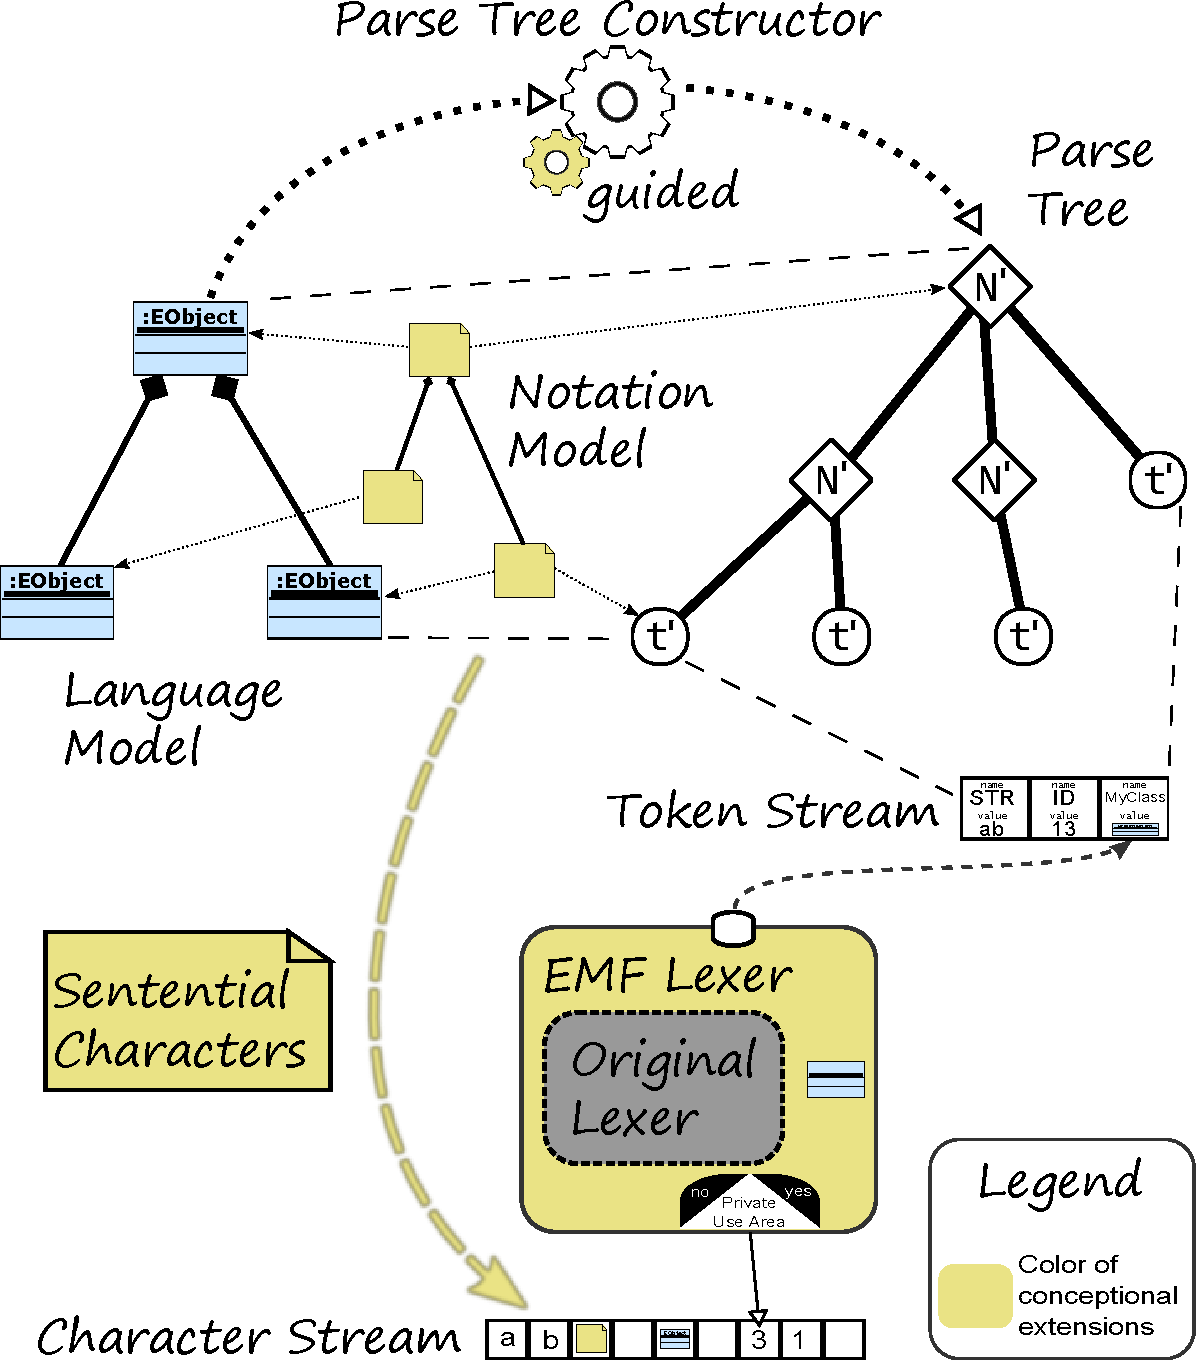
\includegraphics[scale=0.75]{gfx/ex/Concept} 
\caption{Conceptual Overview}
\label{ConceptFigure}
\end{figure}
